\chapter{Training classifier}

\section{Dataset}\label{dataset}
During tuning weigths vector 
All association measures base on statistical data, so in order to obtain reliable results large dataset should be provided.
Machine learning algorithms also need vast and differentiated resources to produce satisfactory result.
Below there are described datasets and its sources which was used for purpose of this thesis.

\subsection{Manually Annotated Subcorpus of NKJP}
Manually annotated subcorpus of NKJP is a part of the National Corpus of Polish, which is a initiative of four institutions: 
Institute of Computer Science at the Polish Academy of Sciences, Institute of Polish Language at the Polish Academy of Sciences, 
Polish Scientific Publishers PWN, and the Department of Computational and Corpus Linguistics at the University of Łódź.
It contains one milion tokens and was manually morfosyntactically "and semantically" annotated by lexicographers. 
Similarly to the main corpus of NKJP it contains text from diverse sources like classic literature, daily newspapers, 
specialist periodicals and journals, transcripts of conversations, and a variety of short-lived and internet texts. 
Manual annotation guarantee correctness of data and it is relatively large what makes it valuable choice for training data.

\subsection{plWordNet Corpus 10.0}

It contains over 4 bilions tokens and it is probably the largest corpus of Polish texts created in controlled way. 
In the article \cite{kgr10} we can find short description of its content: \emph{It consists of IPI PAN Corpus, 
the first annotated corpus of Polish,  National Corpus of Polish, Polish Wikipedia (from 2016), Rzeczpospolita Corpus 
-- corpus of electronic editions of a Polish newspaper from the years 1993-2003, supplemented with text acquired from the Web 
-- only text with small percentage of words unknown to a very comprehensive morphological analyser Morfeusz 2.0 
were included; duplicates were automatically eliminated from the merged corpus.}
Enormous size of this corpus caused computation time to process such amount of information 
long enough to make it impossible to perform tuning weigths and verification of the results on whole corpus. 
That was motivation to utilize only part of that resource. To preserve variety of text, new subcorpus was prepared by randomly picking 
10\% of sentences and dropping rest. Then plain text was annotated by the tager Morphodita\footnote{http://ws.clarin-pl.eu/morphoDiTa.shtml} and stored in CCL format.

\subsection{PLWordNet}
Wordnet is a "lexically-semantic" web, which nodes are lexical units and edges are semantic relations connecting those units.
PLWordNet is the biggest polish wordnet, it was founded by G4.19 Research Group in 2006 and still it is continously developed, 
for now version plWordnet3.1 contains 198000 words, 285000 word's meanings and 670000 semantic relations. Author of this thesis decided to use that resource 
as a source of proper collocations. They were obtained as a set of wccl operators, while MeWeX accepts only MWE listed in file one per line, 
so they had to be preprocessed. This source provided 66853 collocations.

\subsection{Set of relations}
First stage of collocation extraction, selecting candidates, requires set of relations, to reduce number of candidates only to syntactically reasonable. 
These relations has to be in form of WCCL operators. They can specify size of the tuple, part of speech and other properties of phrase element, 
order of tuple or even particular lemma. Set used for purpose of this thesis was taken from resources availble in the MeWeX system. 
At first all relations were used in tuples generation, but examination with use of program \(Cover\) showed that in selected candidates 
there is only 0.44\% of proper collocations. Precise statistics from the output of this program can be found in table \ref{cover_rel_stats}.
Having such large disproportion of positive to negative samples makes training very ineffective. To increase efficacy of learning 
number of incorrect tuples must be reduced. In the table \ref{cover_rel_stats} it is visible, that most of relations have less than 0.05\% 
of positive candidates. Dropping that WCCL operators coverage of proper MWE in generated tuples can be increased to 1.1\%, 
what is still low value, but nevertheless over twice bigger as before. This modification of relation set also greatly shorten computation time 
for all stages following tuples generating, because it decreased number of candidates from 10411380 to 4068265.

\begin{table}[t]
    \centering
    \scriptsize
    \begin{tabular}{|l|r|r|r|}
        \hline 
        \textbf{Relation} & \textbf{MWE} & \textbf{Tuples} & \textbf{Percentage} \\
        \hline
        AdjAdjSubstABC & 1 & 71240 & 0.00140 \\
        AdjAdjSubstABxC & 0 & 22486 & 0.00000 \\
        AdjAdjSubstAxBC & 0 & 117019 & 0.00000 \\
        AdjGenCosAB & 0 & 29 & 0.00000 \\
        AdjGenCosAxB & 0 & 100 & 0.00000 \\
        AdjGenCosBA & 0 & 400 & 0.00000 \\
        AdjGenCosBxA & 0 & 202 & 0.00000 \\
        AdjPrepSubstABC & 30 & 98564 & 0.03044 \\
        AdjPrepSubstABxC & 4 & 73348 & 0.00545 \\
        AdjPrepSubstAxBC & 1 & 99422 & 0.00101 \\
        AdjSubstAdjABC & 31 & 108010 & 0.02870 \\
        AdjSubstAdjABxC & 1 & 119024 & 0.00084 \\
        AdjSubstAdjAxBC & 6 & 78200 & 0.00767 \\
        AdjSubstSubstABC & 27 & 129569 & 0.02084 \\
        AdjSubstSubstABxC & 2 & 198777 & 0.00101 \\
        AdjSubstSubstAxBC & 2 & 79647 & 0.00251 \\
        AgrAdjSubstAB & 2099 & 358130 & 0.58610 \\
        AgrAdjSubstAxB & 437 & 78905 & 0.55383 \\
        AgrAdjSubstBA & 4832 & 183497 & 2.63329 \\
        AgrAdjSubstBxA & 306 & 70984 & 0.43108 \\
        AgrSubstAdjAB & 8159 & 183497 & 4.44639 \\
        AgrSubstAdjAxB & 388 & 70984 & 0.54660 \\
        AgrSubstAdjBA & 1945 & 358130 & 0.54310 \\
        AgrSubstAdjBxA & 606 & 78905 & 0.76801 \\
        AllAdvPartAB & 7 & 22417 & 0.03123 \\
        AllAdvPartAxB & 0 & 14175 & 0.00000 \\
        AllAdvPartBA & 0 & 11715 & 0.00000 \\
        AllAdvPartBxA & 0 & 10347 & 0.00000 \\
        AllBurkSubstAB & 0 & 1426 & 0.00000 \\
        AllBurkSubstAxB & 0 & 981 & 0.00000 \\
        AllBurkSubstBA & 0 & 1402 & 0.00000 \\
        AllBurkSubstBxA & 0 & 1402 & 0.00000 \\
        AllGerQubAB & 292 & 1912 & 15.27197 \\
        AllGerQubAxB & 16 & 2021 & 0.79169 \\
        AllGerQubBA & 56 & 2619 & 2.13822 \\
        AllGerQubBxA & 116 & 4546 & 2.55169 \\
        AllNumSubstAB & 15 & 74696 & 0.02008 \\
        AllNumSubstAxB & 8 & 79706 & 0.01004 \\
        AllNumSubstBA & 4 & 72716 & 0.00550 \\
        AllNumSubstBxA & 6 & 115139 & 0.00521 \\
        AllPartAdvAB & 227 & 11715 & 1.93769 \\
        AllPartAdvAxB & 16 & 10347 & 0.15463 \\
        AllPartAdvBA & 51 & 22417 & 0.22751 \\
        AllPartAdvBxA & 84 & 14175 & 0.59259 \\
        AllQubGerAB & 0 & 2619 & 0.00000 \\
        AllQubGerAxB & 0 & 4546 & 0.00000 \\
        AllQubGerBA & 0 & 1912 & 0.00000 \\
        AllQubGerBxA & 0 & 2021 & 0.00000 \\
        AllSiebieSubstAB & 0 & 2826 & 0.00000 \\
        AllSiebieSubstAxB & 0 & 3303 & 0.00000 \\
        AllSiebieSubstBA & 0 & 1072 & 0.00000 \\
        AllSiebieSubstBxA & 0 & 2465 & 0.00000 \\
        AllSubstBurkAB & 1 & 1402 & 0.07133 \\
        AllSubstBurkAxB & 1 & 1402 & 0.07133 \\
        AllSubstBurkBA & 0 & 1426 & 0.00000 \\
        AllSubstBurkBxA & 0 & 981 & 0.00000 \\
        AllSubstNumAB & 2 & 72716 & 0.00275 \\
        \end{tabular}
        \quad
        \begin{tabular}{|l|r|r| r|}
        \hline 
        \textbf{Relation} & \textbf{MWE} & \textbf{Tuples} & \textbf{Percentage} \\
        \hline
        AllSubstNumAxB & 1 & 115139 & 0.00087 \\
        AllSubstNumBA & 0 & 74696 & 0.00000 \\
        AllSubstNumBxA & 0 & 79706 & 0.00000 \\
        AllSubstSiebieAB & 4 & 1072 & 0.37313 \\
        AllSubstSiebieAxB & 1 & 2465 & 0.04057 \\
        AllSubstSiebieBA & 1 & 2826 & 0.03539 \\
        AllSubstSiebieBxA & 1 & 3303 & 0.03028 \\
        AllSubstSubstAB & 2410 & 931272 & 0.25879 \\
        AllSubstSubstAxB & 588 & 1388050 & 0.04236 \\
        AllSubstSubstBA & 569 & 931272 & 0.06110 \\
        AllSubstSubstBxA & 1011 & 1388050 & 0.07284 \\
        AllVerbSiebieAB & 9050 & 11393 & 79.43474 \\
        AllVerbSiebieAxB & 2339 & 3526 & 66.33579 \\
        AllVerbSiebieBA & 6233 & 8839 & 70.51703 \\
        AllVerbSiebieBxA & 3943 & 6211 & 63.48414 \\
        CosAdjGenAB & 1 & 400 & 0.25000 \\
        CosAdjGenAxB & 0 & 202 & 0.00000 \\
        CosAdjGenBA & 0 & 29 & 0.00000 \\
        CosAdjGenBxA & 0 & 100 & 0.00000 \\
        GndAdjSubstAB & 21 & 3896 & 0.53901 \\
        GndAdjSubstAxB & 71 & 14057 & 0.50509 \\
        GndAdjSubstBA & 51 & 7862 & 0.64869 \\
        GndAdjSubstBxA & 49 & 16888 & 0.29015 \\
        GndSubstAdjAB & 70 & 7854 & 0.89127 \\
        GndSubstAdjAxB & 55 & 16888 & 0.32568 \\
        GndSubstAdjBA & 19 & 3886 & 0.48893 \\
        GndSubstAdjBxA & 96 & 14057 & 0.68293 \\
        Ppron3GenSubstAB & 1 & 8764 & 0.01141 \\
        Ppron3GenSubstAxB & 0 & 6563 & 0.00000 \\
        Ppron3GenSubstBA & 0 & 4613 & 0.00000 \\
        Ppron3GenSubstBxA & 0 & 7406 & 0.00000 \\
        SubstAdjAdjABC & 13 & 32151 & 0.04043 \\
        SubstAdjAdjABxC & 0 & 91908 & 0.00000 \\
        SubstAdjAdjAxBC & 0 & 25040 & 0.00000 \\
        SubstAdjSubstABC & 44 & 156730 & 0.02807 \\
        SubstAdjSubstABxC & 2 & 151333 & 0.00132 \\
        SubstAdjSubstAxBC & 8 & 209355 & 0.00382 \\
        SubstAdvAdjABC & 4 & 13318 & 0.03003 \\
        SubstAdvAdjABxC & 11 & 8651 & 0.12715 \\
        SubstAdvAdjAxBC & 1 & 23663 & 0.00423 \\
        SubstConjSubstABC & 20 & 81567 & 0.02452 \\
        SubstConjSubstABxC & 7 & 57989 & 0.01207 \\
        SubstConjSubstAxBC & 7 & 53419 & 0.01310 \\
        SubstPpron3GenAB & 0 & 4613 & 0.00000 \\
        SubstPpron3GenAxB & 0 & 7406 & 0.00000 \\
        SubstPpron3GenBA & 0 & 8764 & 0.00000 \\
        SubstPpron3GenBxA & 0 & 6563 & 0.00000 \\
        SubstPrepSubstABC & 120 & 221630 & 0.05414 \\
        SubstPrepSubstABxC & 12 & 143286 & 0.00837 \\
        SubstPrepSubstAxBC & 19 & 183775 & 0.01034 \\
        SubstSubstAdjABC & 46 & 98007 & 0.04694 \\
        SubstSubstAdjABxC & 0 & 76129 & 0.00000 \\
        SubstSubstAdjAxBC & 8 & 147898 & 0.00541 \\
        SubstSubstSubstABC & 13 & 88445 & 0.01470 \\
        SubstSubstSubstABxC & 2 & 149396 & 0.00134 \\
        SubstSubstSubstAxBC & 2 & 155425 & 0.00129 \\
        \hline
        Sum & 46703 & 10411380 & 0.44857 \\
        \hline
    \end{tabular} 
    \caption{Coverage of proper collocations per relation}
    \label{cover_rel_stats}
\end{table}

\section{Methods used for training}
To train vector of weigths PSO algorithm with modifications described in section \ref{pso_improv} was used. 
Dataset used for learning was both Manually Annotated Subcorpus of NKJP and plWordNet Corpus 10.0. Tuples were generated using reduced set of relations
to increase its efficiency and shorten computation time.

To select proper size of the swarm, short reaserch was conducted on NKJP Subcorpus only, to analyze influence of the number of particles on 
algortihm efficacy. Test was carried out for sizes: 5, 10, 20, 40 and accordingly 4000, 2000, 1000, 500 iterations, 
to preserve the same number of particle evaluations and as a result the same computation time.
Also parameters \(\omega, \omega _l, \omega _g\), were choosen in similar way, by training on small data, with different configurations, 
to select the best found set of values.

Final values that were choosen for training were: \\
\[
\omega = 1.0, \quad
\omega _l = 0.2, \quad
\omega _g = 0.8, \quad
swarm\_size = 40
\]

Measure of quality, that were used as a target for an optimization is Average Precision. It is precisely described in section \ref{ap_desc}.
\section{Results}
Figure \ref{pso_train} presents to process of training showing value of best achieved Average precision value for given iteration.
From the beggining ut to 300 iteration aggregator achieves average score, comparable to aquired by other association measures. 
Next iterations bring vast improvement, quality of the result increases quickly till 1250 iteration, where it reaches the maximum 
obtained by this algorithm. Final returned value of Average Precision is 0.673891.


\begin{figure}[ht]
    \centering
    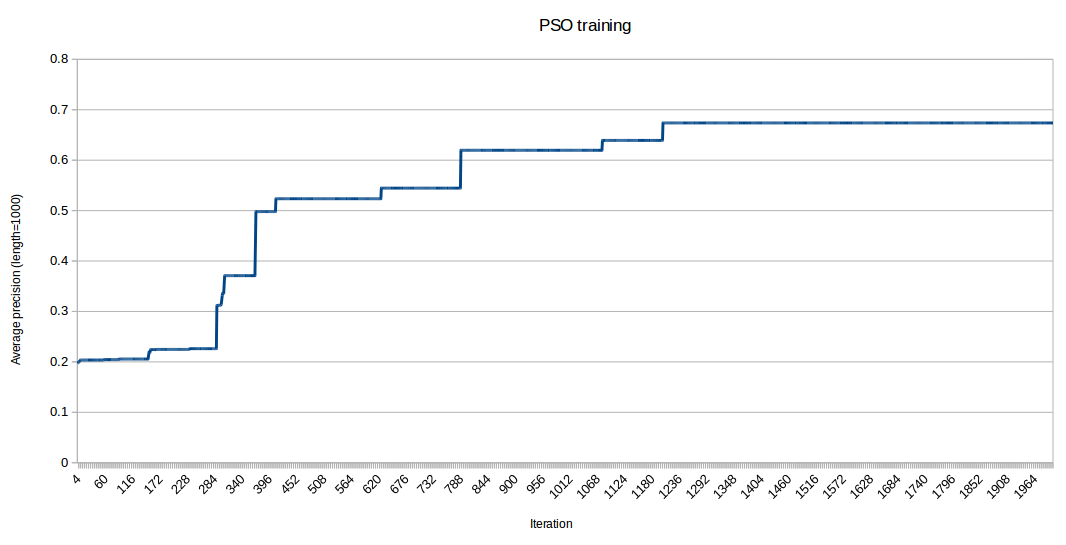
\includegraphics[scale=0.45]{img/pso_train.png}
    \caption{Flow chart of Particle Swarm Optimization}
    \label{pso_train}
\end{figure}